%--- mutation

\section{Mutation}
\label{sec:mutation}

Der Fokus auf die Mutation ist das entscheidende Merkmal von Evolutionsstrategien.

Während die Selektion von Elternindividuen zur Erzeugung von Nachkommen und die evtl. durchgeführte Rekombination anhand der statistischen Gleichverteilung stattfinden, wird die Mutation nach der statistischen Normalverteilung vollzogen.

Statistische Gleichverteilung bedeutet, dass jedes Individuum bei der Selektion der Eltern mit der gleichen Wahrscheinlichkeit ausgewählt werden kann. Die Selektion ist somit unabhängig von der Qualität der Individuen. Dieses Verfahren wird auch bei der Selektion der Vektorwerte bei der Rekombination von zwei Elternindividuen verwendet.

Bei der Mutation hingegen kommt die Normalverteilung zum Einsatz. Dabei ist es wahrscheinlicher, dass eine Zufallsvariable seine Ausprägung nah am Erwartungswert hat. Werte, die weit vom Erwartungswert entfernt sind, sind relativ unwahrscheinlich, je nach Standardabweichung.

In den folgenden Kapiteln wird beschrieben, welchen Grundsatz diese Funktionsweise verfolgt und wie die Mutation im Pseudocode umgesetzt werden kann.
Zunächst werden die mathematischen Grundlagen der Normalverteilung kurz aufgegriffen.

\subsection{Normalverteilung}

Die Normal- bzw. Gauß-Verteilung ist ein wichtiger Typ stetiger Wahrscheinlichkeitsverteilungen.
Stetig bezieht sich in dem Zusammenhang auf die Zufallsvariablen, die in einem beliebigen Intervall eine unendliche Menge an Werten annehmen können.
Als Gegenspieler gibt es diskrete Zufallsvariablen, die eine abzählbare Menge an Ausprägungen in einem Intervall darstellen.

Die wichtigen Kennwerte von Wahrscheinlichkeitsverteilungen sind \enquote{Mittelwert}, \enquote{Varianz} und \enquote{Standardabweichung}.

Als Mittelwert $m$ wird das arithmetische Mittel aller möglichen Ausprägungen der Zufallsvariablen definiert. Dieses wird über die Summe aller Werte geteilt durch die Anzahl $n$ an Ausprägungen bestimmt: $m = \frac{1}{n} \sum_{i=1}^n a_i$

Die Varianz sowie die Standardabweichung geben die Schwankung der Werte von dem Erwartungswert an.

Die Varianz $s^2$ wird mit folgender Formel gebildet: $s^2 = \frac{1}{n} \sum_{i=1}^n (a_i-m)^2$.

Die Standardabweichung $s$ entspricht somit der Wurzel der Varianz: $s = \sqrt{s^2} = \sqrt{\frac{1}{n} \sum_{i=1}^n (a_i-m)^2}$.

Die Normalverteilung wird anhand des Mittelwerts und der verwendeten Standardabweichung notiert: $N(m, \sigma)$

Die Verteilungsfunktion der Normalverteilung ist durch $f(x) = \frac{1}{\sqrt{2 \pi \sigma^2}} \int_{-\infty}^x e^{-\frac{(x-m)^2}{2 \sigma^2}} dx$ gegeben. Sie gibt an, zu welcher Wahrscheinlichkeit f(x) der Wert die Ausprägung $\le x$ ist.

\begin{figure}[H]
\centering
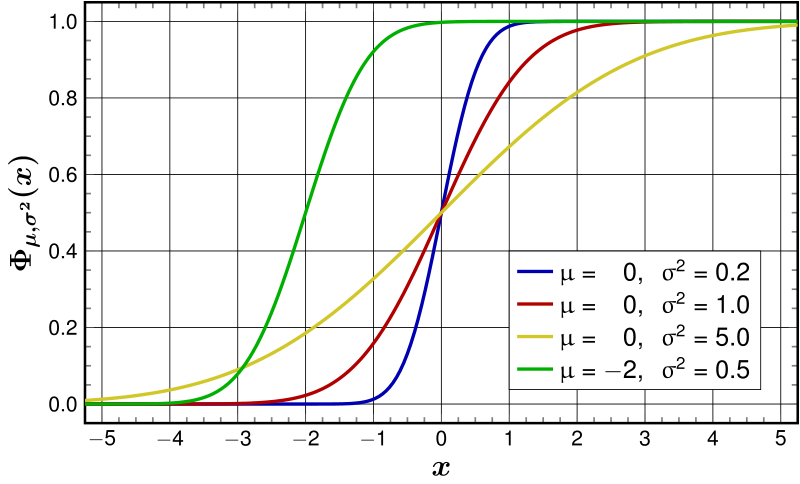
\includegraphics[width=0.75\textwidth]{img/Verteilungskurven.png}
\caption[Verteilungsfunktionen]{Verteilungsfunktionen\protect\footnotemark}
\label{fig:verteilungskurven}
\end{figure}
\footnotetext{\url{https://upload.wikimedia.org/wikipedia/commons/thumb/7/74/Normal-distribution-cumulative-density-function-many.svg/800px-Normal-distribution-cumulative-density-function-many.svg.png}}

Die Dichtefunktion bzw. die Wahrscheinlichkeitsdichte der Normalverteilung ergibt sich aus der Ableitung $F'(x)$ der Verteilungsfunktion $f(x)$ und ist eine Glockenkurve. Deren Streckung bzw. Stauchung lässt sich anhand der Standardabweichung einstellen. Die x-Achsenverschiebung wird durch den Erwartungswert vorgenommen\footnote{\textit{siehe} Tool zur Visualisierung: \url{https://www.geogebra.org/m/e2Ppkaj9}}. Abbildung \ref{fig:glockenkurven} veranschaulicht unterschiedliche Dichtefunktionen von Normalverteilungen.

\begin{figure}[H]
\centering
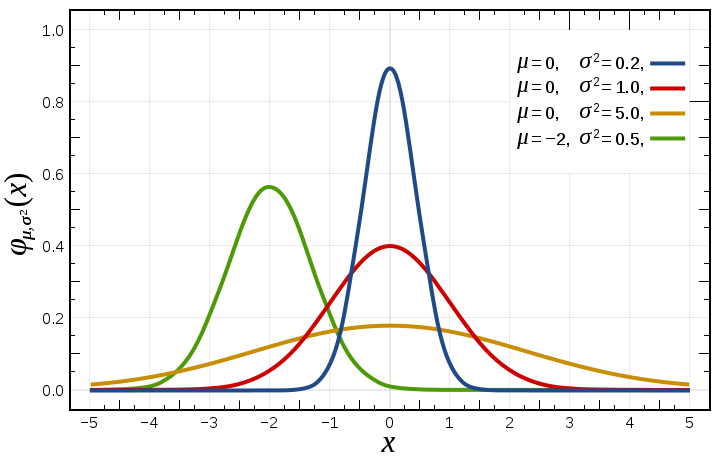
\includegraphics[width=0.75\textwidth]{img/Glockenkurven.png}
\caption[Dichtefunktionen]{Dichtefunktionen\protect\footnotemark}
\label{fig:glockenkurven}
\end{figure}
\footnotetext{\url{https://upload.wikimedia.org/wikipedia/commons/thumb/7/74/Normal_Distribution_PDF.svg/720px-Normal_Distribution_PDF.svg.png}}

Die Dichtefunktion lautet: $f(x) = \frac{1}{\sqrt{2 \pi \sigma^2}} e^{-\frac{(x-m)^2}{2 \sigma^2}}$. Eine Teilfläche unterhalb der Dichtefunktion beschreibt die Wahrscheinlichkeit, dass eine Zufallsvariable eine Ausprägung in dem festgelegten Bereich annimmt. Sie wird errechnet durch die Formel: $P(x_1 \le X \le x_2) = \int_{x_1}^{x_2} f(x) dx$

\subsection{Standardnormalverteilung}

Jede Normalverteilung lässt sich mithilfe der Substitution $z = \frac{x - \mu}{\sigma}$ zur in die Standardnormalverteilung überführen.
Da eine eigenhändige Berechnung ohne Hilfsmittel sehr aufwändig ist, wird dieser Trick angewendet, um die Wahrscheinlichkeiten anhand einer vorgefertigten Standardnormalverteilungstabelle abzulesen:

$F(x) = W(X \le x) = \Phi(\frac{x - \mu}{\sigma}) = \Phi(z)$

\subsection{Mutative Schrittweitenregelung}

Die Idee der mutativen Schrittweitenregelung ist es nun, die reellen Vektorwerte eines Individuums bei der Mutation anhand von Zufallszahlen der $N(0, \sigma)$-Verteilung in jeder Generation anzupassen. Da der Mittelwert $0$ ist, werden hauptsächlich kleine Änderungen vorgenommen. Es gibt jedoch keine bestimmte Suchrichtung. Die Schrittweite der Mutation kann über die Standardabweichung konfiguriert werden. Es werden also positive und negative Zahlen auf die Vektorwerte addiert. Jeder Vektorwert wird um eine neue Zufallszahl aus dieser Verteilung verändert.

$x_{neu} = x_{alt} + N(0, \sigma)$

Nach einer analytischen Untersuchung von einfachen Qualitätsfunktionen zur Analyse der optimalen Streuung der Zufallszahlen ermittelte Rechenberg anhand des \enquote{Korridor}- und des \enquote{Sphären}-Modells, dass die optimale Streuung ungefähr $\frac{1}{5}$ beträgt. Insofern solle der Anteil an erfolgreichen Mutationen zur Verbesserung der Qualität des betroffenen Individuums über mehrere Generationen durchschnittlich mindestens $\frac{1}{5}$ betragen. Wird dieser Wert unterschritten, so wird die Streuung bzw. Standardabweichung erhöht. Wird er überschritten, wird die Streuung verringert.

Die Regeln der Anpassung der Schrittweite (Standardabweichung) je nach Erfolgs- bzw. Verbesserungsrate ergeben sich somit als:
\begin{enumerate}
	\item $\sigma(x+n) = c \cdot \sigma(x)\ |\ p > \frac{1}{5}$
    \item $\sigma(x+n) = d \cdot \sigma(x)\ |\ p < \frac{1}{5}$
    \item $\sigma(x+n) = \sigma(x)\ |\ p = \frac{1}{5}$
\end{enumerate}

Laut Schwefel empfiehlt es sich, $c = 1,22$ und $d = 0,82$ zu verwenden.

Durch die Anpassung der Schrittweite wird also je nach Anteil an erfolgreichen Mutationen die Standardabweichung angepasst, was dazu führt, dass die Zufallszahlen zur Mutation der Vektorwerte des Individuums je nach Veränderung noch wahrscheinlicher an $0$ bzw. etwas weiter entfernt von $0$ liegen und somit die Veränderung des gesamten Individuums in kleinerem bzw. größeren Maße geschieht.

Im Pseudocode sieht der Vorgang entsprechend so aus:

\begin{lstlisting}[caption={Mutative Schrittweitenregelung}\label{lst:mutative_schrittweitenrgelung_es}, firstnumber=1, captionpos=b, label=code:mutative_schrittweitenrgelung_es]
<@\colorcodeline{algorithm mutation(individuen[1,...,$\mu$], $\sigma$, n)}@>
	mutierteIndividuen <- []
	for i <- 1...$\mu$
		individuum <- individuen[i]
		mutiertesIndividuum <- []		
			for j <- 1,..,n
				z <- Zufallszahl $\in$ $N(0, \sigma)$
				mutiertesIndividuum[j] <- individuum[j] + z
		mutierteIndividuen <- mutierteIndividuen + mutiertesIndividuum
	return mutierteIndividuen
	
<@\colorcodeline{algorithm berechneAnteilVerbesserungen}@>(startIndividuen[1,...,$\mu$], mutierteIndividuen[1,...,$\mu$])
	verbesserungen <- 0	
	for i <- 1...$\mu$
		if qualitaet(mutierteIndividuen[i]) > qualitaet(startIndividuen[i])
			verbesserungen <- verbesserungen + 1
	return verbesserungen / $\mu$
	
<@\colorcodeline{algorithm passeStandardabweichungAn($\sigma$, p)}@>
	c <- 1.22
	d <- 0.82
	if p > $\frac{1}{5}$
		return c * $\sigma$
	else if p < $\frac{1}{5}$
		return d * $\sigma$
	else
		return $\sigma$

<@\colorcodealgorithm{algorithm Mutative-Schrittweitenregelung-ES()}@>
	iterationsLimit <- x $\in \mathbb{N}$
	generationszaehler <- 0
	anzahl_eltern <- $\mu \ge 1$
	anzahl_kinder <- $\lambda \ge$ anzahl_eltern
	<@\colorcodeline{standardabweichung <- $\sigma$ $\in$ $\mathbb{R}$}@>
	wunschqualitaet <- y $\in \mathbb{R}$
	individuengroesse <- n $\in \mathbb{N}$
	population <- baue_population($\mu$, individuengroesse)
	while qualitaet(population) < wunschqualitaet and generationszaehler < iterationslimit
		generationszaehler <- generationszaehler + 1
		eltern <- elternSelektion(population, anzahl_kinder)
		kinder <- duplikation(eltern, individuengroesse)
		<@\colorcodeline{mutierte\_kinder}@> <- mutation(kinder, standardabweichung, individuengroesse)
		<@\colorcodeline{erfolgreiche\_mutationen}@> <- berechneAnteilVerbesserungen(kinder, mutierte_kinder)
		<@\colorcodeline{standardabweichung}@> <- passeStandardabweichungAn(standardabweichung, erfolgreiche_mutationen)
		population <- selektion(mutierte_kinder, $\mu$, qualitaet)
	loesung <- bestenSelektion(population)
\end{lstlisting}

\subsection{Selbstregulierende Schrittweitenanpassung je Vektorwert}

Zuvor resultierten die Zufallszahlen für jeden Vektorwert eines Individuums aus der $N(0, \sigma)$-Verteilung. Allerdings ist es nicht zwangsläufig klug, eine Schrittweite für alle Parameter des Individuums zu nutzen. Da man die optimalen Schrittweiten nicht im Vorhinein vorhersagen kann, besteht die Hoffnung, dass sich die Schrittweite während der Evolution selbstständig entwickelt. Nun besteht ein Individuum also aus einem Vektor aus Tupeln, welches jedem Vektorwert eine Standardabweichung zuordnet: $<x, \sigma> = <(x_1,...,x_n), (\sigma_1,...,\sigma_n)>$. Bei der Rekombination können die Werte eines Tupels jeweils zufällig aus einem der Elternindividuen stammen. Als alternatives Rekombinationsschema kann der Mittelwert der Eltern für den Nachwuchs übernommen werden.

Die Standardabweichung zu jedem Vektorwert wird angepasst, indem sie mit einer Exponentialfunktion multipliziert wird, welche die normalverteilte Zufallszahl beinhaltet: $\sigma_{neu} = \sigma_{alt} \cdot e^{N(0, \Delta)}$. Dadurch wird die Standardabweichung nur mit einer positiven reellen Zahl größer als $1$ multipliziert. $\Delta$ beschreibt die Größe der Anpassung der Schrittweite und kann frei gewählt werden. Er beeinflusst die vorliegende Normalverteilung und somit die generierten Zufallszahlen. Der neue Wert wird wie gehabt angepasst, wobei nun die zu addierende Zufallszahl durch die neue Standardabweichung beeinflusst wird: $x_{neu} = x_{alt} + N(0, \sigma_{neu})$.

Nach Rechenberg gibt es eine weitere Empfehlung, wie die Vektorkomponenten mutiert werden können. Dabei wird die Anzahl an Generationen berücksichtigt: $x_{neu} = x_{alt} + $Schrittweite $\cdot N(0, \frac{1}{\sqrt{n}})$. Die Schrittweite ist in diesem Fall die eigentliche Schrittweite $x$ skaliert um $y$: $Schrittweite = x \cdot y$. Für jedes der zu mutierenden Individuen wird bestimmt, ob $y$ um den Faktor $1,5$ erhöht oder mit dem Faktor $\frac{1}{1,5}$ verringert wird.

Der folgende Pseudocode stellt die erste Variante der Schrittweitenanpassung für jeden Vektorwert dar.

\begin{lstlisting}[caption={Selbstregulierende Schrittweitenanpassung je Vektorwert}\label{lst:selbstregulierende_schrittweitenanpassung_es}, firstnumber=1, captionpos=b, label=code:selbstregulierende_schrittweitenanpassung_es]
<@\colorcodeline{algorithm baue\_individuum(n, $\sigma$)}@>
	individuum <- []
	for _ <- 1...n
		individuum <- individuum + (zufälliges $x \in \mathbb{R}$, $\sigma$)
	return individuum
	
<@\colorcodeline{algorithm baue\_population($\mu$, n, $\sigma$)}@>
	population <- []
	for i <- 1...$\mu$
		individuum <- baue_individuum(n, $\sigma$)
		population <- population + individuum
	return population

<@\colorcodeline{algorithm mutation(individuen[1,...,$\mu$], $\Delta$, n)}@>
	mutierteIndividuen <- []
	for i <- 1...$\mu$
		// ($x_i$, $\sigma_i$) = (0, 1)
		individuum <- individuen[i]
		mutiertesIndividuum <- []
			for j <- 1,..,n
				skalierung_standardabweichung_exponent <- Zufallszahl $\in$ $N(0, \Delta)$
				skalierung_standardabweichung <- e^skalierung_standardabweichung_exponent
				mutiertesIndividuum[j][0] <- individuum[0] * skalierung_standardabweichung
				z <- Zufallszahl $\in$ $N(0,$ mutiertesIndividuum[j][0]$)$
				mutiertesIndividuum[j][1] <- individuum[1] + z
		mutierteIndividuen <- mutierteIndividuen + mutiertesIndividuum
	return mutierteIndividuen

<@\colorcodealgorithm{algorithm Mutative-Schrittweitenregelung-ES()}@>
	iterationsLimit <- x $\in \mathbb{N}$
	generationszaehler <- 0
	anzahl_eltern <- $\mu \ge 1$
	anzahl_kinder <- $\lambda \ge$ anzahl_eltern
	<@\colorcodeline{schrittweitenanpassung <- $\Delta$ $\in$ $\mathbb{R}$}@>
	wunschqualitaet <- y $\in \mathbb{R}$
	individuengroesse <- n $\in \mathbb{N}$
	population <- baue_population($\mu$, individuengroesse)
	while qualitaet(population) < wunschqualitaet and generationszaehler < iterationslimit
		generationszaehler <- generationszaehler + 1
		eltern <- elternSelektion(population, anzahl_kinder)
		kinder <- duplikation(eltern, individuengroesse)
		mutierte_kinder <- mutation(kinder, <@\colorcodeline{schrittweitenanpassung}@>, individuengroesse)
		population <- selektion(mutierte_kinder, $\mu$, qualitaet)
	loesung <- bestenSelektion(population)
\end{lstlisting}

Nur eine geeignete Mutationsstrategie und eine gute Schrittweitenanpassung garantieren den Erfolg der Evolutionsstrategie.
Die Schrittweite liegt in der Regel in einem recht kleinen \enquote{Evolutionsfenster}, innerhalb dessen die Fortschrittsgeschwindigkeit der Evolution am höchsten ist. Außerhalb nimmt sie sehr stark ab.
